The Park transform, also known as the \( dq \) transformation, is another
fundamental mathematical tool used in the analysis of three-phase electric
machines.In the late 1920s, R.H. Park\cite{R. H. Park} introduced a new
approach to electric machine analysis. He formulated a change of variables
which replaced variables such as voltages, currents, and flux linkages
associated with fictitious windings rotating with the rotor. He referred the
stator and rotor variables to a reference frame fixed on the rotor. From the
rotor point of view, all the variables can be observed as constant values
\subsection{What is Park Transform?}

The Park transform shifts the perspective from the traditional stationary
reference frame to a rotating reference frame that moves with the rotor. This
transformation effectively decouples the complex interactions between variables
such as voltages, currents, and flux linkages that occur in three-phase
systems. By aligning with the rotor's magnetic field, the transform separates
these variables into two orthogonal components: \( d \) (direct) and \( q \)
(quadrature). Figure:\ref{fig:Park Transform}

In practical terms, within the \( dq \) frame, \( d \) represents the component
aligned with the rotor flux (direct axis), while \( q \) represents the
component perpendicular to the rotor flux (quadrature axis). This separation
facilitates independent control of the torque-producing and magnetizing
currents in field-oriented control strategies, essential for optimizing the
performance of electric machines.\begin{figure}[h]
    \centering
    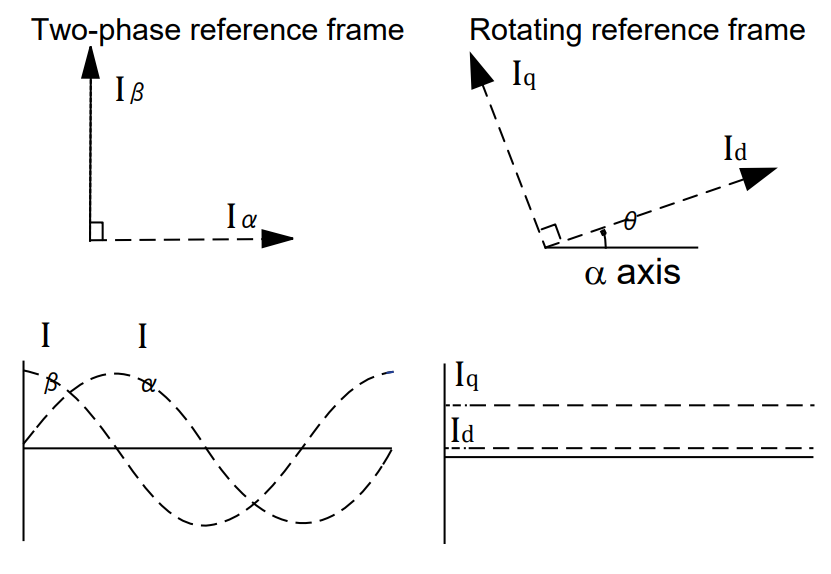
\includegraphics[width=0.6\textwidth]{park-clarke.png}
    \caption{Park Transform}
    \label{fig:Park Transform}
\end{figure}

To derive the Park transformation matrix, we first define the transformation
angle \( \theta \), which corresponds to the rotor angle. By applying an axis
rotation and rotating the Clarke frame by \( \theta \), we obtain the
transformation matrix \( T_{dq0} \).

\( T_{dq0} \) is given by:

\begin{equation*}
    T_{dq0} =
    \begin{bmatrix}
        \cos \theta & -\sin \theta & 0 \\
        \sin \theta & \cos \theta  & 0 \\
        0           & 0            & 1
    \end{bmatrix}
\end{equation*}

\begin{figure}[h]
    \centering
    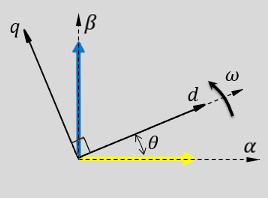
\includegraphics[width=0.4\textwidth]{park-coordinate.png}
    \caption{Park Frame of reference}
    \label{fig:Park Frame of reference}
\end{figure}
\subsection{Derivation of the Park Transform Matrix}

\noindent
Where \( \theta \) is the electrical angle of the rotor position.
\noindent
The Park transform equations for transforming the three-phase quantities \(
V_\alpha, V_\beta, V_0 \) to the \( dq \) frame are:

\begin{equation*}
    V_d = V_\alpha \cos \theta + V_\beta \sin \theta
\end{equation*}
\begin{equation*}
    V_q = -V_\alpha \sin \theta + V_\beta \cos \theta
\end{equation*}
\begin{equation*}
    V_0 = V_0
\end{equation*}
\noindent
Converting these equations into matrix form, we get:

\begin{equation*}
    \begin{bmatrix}
        V_d \\
        V_q \\
        V_0
    \end{bmatrix}
    =
    \begin{bmatrix}
        \cos \theta & -\sin \theta & 0 \\
        \sin \theta & \cos \theta  & 0 \\
        0           & 0            & 1
    \end{bmatrix}
    \begin{bmatrix}
        V_\alpha \\
        V_\beta  \\
        V_0
    \end{bmatrix}
\end{equation*}
or in the shorthand notation:
\begin{equation*}
    V_{dq0} = T_{dq0} V_{\alpha\beta0}
\end{equation*}

Where:
\begin{equation*}
    V_{dq0} = \begin{bmatrix}
        V_d \\
        V_q \\
        V_0
    \end{bmatrix}
\end{equation*}
\begin{equation*}
    V_{\alpha\beta0} = \begin{bmatrix}
        V_\alpha \\
        V_\beta  \\
        V_0
    \end{bmatrix}
\end{equation*}
\begin{equation*}
    T_{dq0} =
    \begin{bmatrix}
        \cos \theta & -\sin \theta & 0 \\
        \sin \theta & \cos \theta  & 0 \\
        0           & 0            & 1
    \end{bmatrix}
\end{equation*}
